\subsection{Геометрия масс}

\subsubsection*{11.8(7)}
Запишем тензор квадрата расстояния
\begin{equation}
\label{t1}
    \widetilde{r_i}\T \widetilde{r_i} = \begin{pmatrix}
        y_i^2 + z_i^2 & -x_i y_i & - x_i z_i \\
        -x_i y_i & x_i^2 + y_i^2 & - y_i z_i \\
        -x_i z_i & -y_i z_i & x_i^2 + y_i^2 \\
    \end{pmatrix} = \hat j_i,
\end{equation}
суммируя, получим
\begin{equation}
\label{t2}
    \hat J_0 = \begin{pmatrix}
        J_x & - J_{xy} & -J_{xz} \\
        -J_{xy} & J_y & -J_{yz} \\
        -J_{xz} & -J_{yz} & J_z \\
    \end{pmatrix}.
\end{equation}
В силу симметрии системы $J_x = J_y = J_z$, выбрав сферические координаты найдём $J_z$:
\begin{equation}
\label{t3}
    J_z = \int_M (y^2 + x^2) \d m = \rho \int_V (y^2 + x^2) \d V =
    \rho \int\limits_0^R \int\limits_0^{2\pi} \int\limits_0^{\pi/2} r^4 \sin^3 \theta \d r \d \varphi \d \theta = 
    \frac{2}{5} R^5 \frac{1}{R^2}  \left(\frac{4}{3} R^3 \rho \pi \right) = \frac{2}{5} M R^2.
\end{equation}


\subsubsection*{11.12}
Тензор инерции твердого тела в базисе $(\vc{e}_1, \vc{e}_2, \vc{e}_3)$ имеет такой вид
\begin{equation*}
    \hat{J} = \begin{pmatrix}
        A & 0 & 0 \\
        0 & B & -D \\
        0 & -D & C \\
    \end{pmatrix}, \hspace{0.5cm} D \neq 0.
\end{equation*}
Хотелось бы его к диагональному виду привести. 
Повернем оси вокруг оси $Ox$ на некоторый угол $\alpha$ и приведём к диагональному виду
\begin{equation*}
    S\T \hat{J} S = \dmat{3}{A'}{B'}{C'}, \hspace{1cm} 
    S = \begin{pmatrix}
        1 & 0 & 0 \\
        0 & \cos \alpha & \sin \alpha \\
        0 & -\sin \alpha & \cos \alpha \\
    \end{pmatrix}.
\end{equation*}
После нескольких монотонных операций (ограничив все на плоскость $Oxy$) получаем
\begin{equation*}
    S\T J S \bigg|_{Oyz} = 
    \begin{pmatrix}
            B \cos ^2 \alpha + C \sin^2 \alpha + D \sin 2\alpha &
            B \sin 2 \alpha / 2 - C \sin 2 \alpha / 2 - D \cos 2 \alpha \\
            B \sin 2 \alpha / 2 - C \sin 2 \alpha / 2 - D \cos 2 \alpha &
            B \cos ^2 \alpha + C \cos^2 \alpha - D \sin 2\alpha \\
    \end{pmatrix},
\end{equation*}
откуда находим $\alpha$ 
\begin{equation*}
    \cos 2\alpha = \frac{B-C}{\sqrt{4D^2+(B-C)^2}}
\end{equation*}
и, соответсвенно,
\begin{equation}
    A' = A, \hspace{0.5cm} 
    B' = \frac{1}{2} \left(
        B + C + \sqrt{(B-C)^2+4D^2}
    \right), \hspace{0.5cm} 
    C' = \frac{1}{2} \left(
        B + C - \sqrt{(B-C)^2+4D^2}
    \right).
\end{equation}
Направляющие же векторы найдём, повернув базисные векторы, 
\begin{equation*}
    S \begin{pmatrix}
        \vc{e}_2 \\ \vc{e}_3
    \end{pmatrix} = 
    \begin{pmatrix}
        \vc{e}_2' \\ \vc{e}_3'
    \end{pmatrix},
    \hspace{0.5cm} \Rightarrow \hspace{0.5cm} 
    \left\{\begin{aligned}
        \vc{e}_2' &= (\vc{e}_2 + \tg \alpha \vc{e}_3) / n_2, \\
        \vc{e}_3' &= (-\tg \alpha \vc{e}_2 + \vc{e}_3) / n_3
    \end{aligned}\right.
\end{equation*}
Возвращаясь в трёхмерие наш новый базис (который остается отнормировать)
\begin{equation}
    \vc{e}_1' = \left(1,\ 0,\ 0\right), \hspace{0.5cm} 
    \vc{e}_2' = \left(0,\ D,\ (B'-B)\right), \hspace{0.5cm} 
    \vc{e}_3' = \left(0,\ C'-C,\ D\right).
\end{equation}


\subsubsection*{11.18}


\begin{figure}
    % \begin{center}
        \begin{minipage}[b]{0.3\textwidth}
            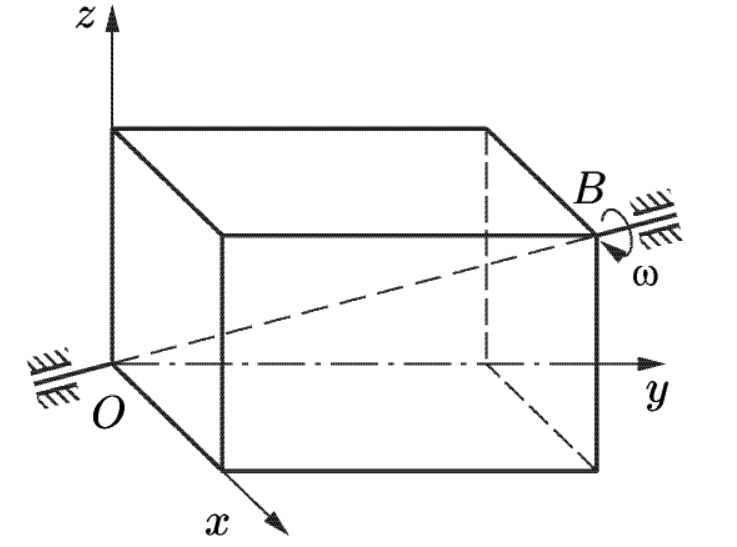
\includegraphics[width=0.99\textwidth]{figures/1.png}
            \caption{К задаче 11.18}
        \end{minipage}
        \hspace{0.5cm} 
        \begin{minipage}[b]{0.35\textwidth}
            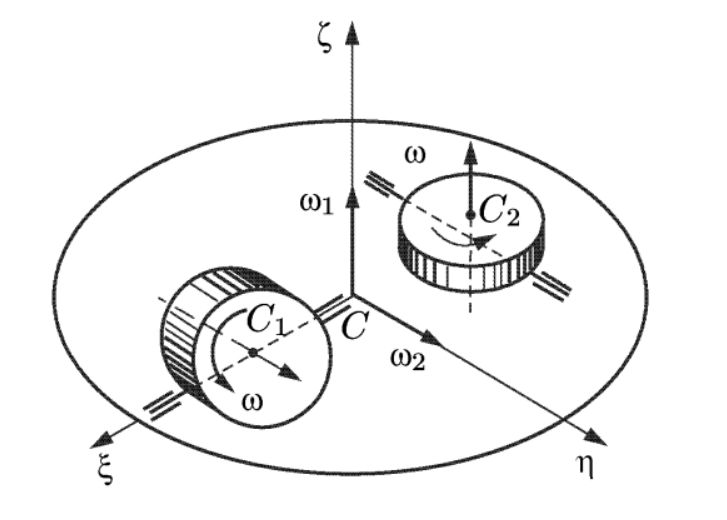
\includegraphics[width=0.9\textwidth]{figures/2.png}
            \caption{К задаче 11.27}
        \end{minipage}
        \hspace{0.5cm} 
        \begin{minipage}[b]{0.35\textwidth}
            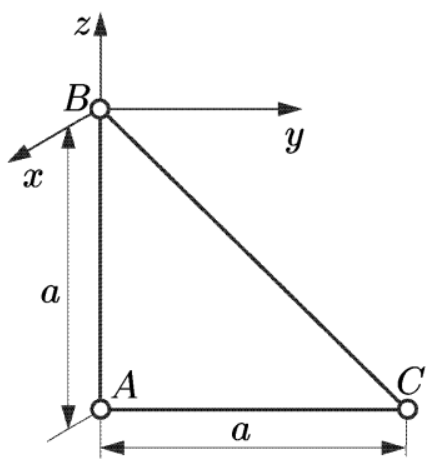
\includegraphics[width=0.65\textwidth]{figures/3.png}
            \caption{К задаче 11.27}
        \end{minipage}
    % \end{center}
\end{figure}


Поместим начало координат в центр масс (потому что так привычнее считать) и найдём тензор инерции по \eqref{t1} и \eqref{t2}, аналогично \eqref{t3}, несколько раз проинтегрировав по параллелепипеду 
\begin{align*}
    J_z = \rho \int_V (x^2 + y^2) \d V = \rho 
    \int\limits_{-a/2}^{a/2} \hspace{-2.5 mm} d x \hspace{-1.0 mm}
    \int\limits_{-b/2}^{b/2} \hspace{-2.5 mm} d y \hspace{-1.0 mm}
    \int\limits_{-c/2}^{c/2} \hspace{-2.5 mm} d z 
    \ (x^2 + y^2) = \frac{1}{12} m (a^2 + b^2),
\end{align*}
аналогичные результаты получим для $J_y, J_x$
\begin{equation*}
    J_y = \ \ldots \ = \frac{1}{12} m (a^2 + c^2),
    \hspace{1cm} 
    J_x = \ \ldots \ = \frac{1}{12} m (b^2 + c^2).
\end{equation*}
Остается найти осевые моменты инерции
\begin{equation*}
    J_{xy} = \rho \int_V x y \d V = \rho \frac{1}{16} a^2 b^2 c^2 = \frac{1}{16} m a b,
    \hspace{0.5cm} 
    J_yz = \ \ldots \ = \frac{1}{16} mbc,
    \hspace{0.5cm} 
    J_xz = \ \ldots \ = \frac{1}{16} mac.
\end{equation*}
Таким образом
\begin{equation}
    \hat{J}_O = \frac{1}{48} m 
    \begin{pmatrix}
        4(b^2+c^2) & -3ab & -3ac \\
        -3ab & 4(a^2+c^2) & -3bc \\
        -3ac & -3bc & 4(a^2+b^2) \\
    \end{pmatrix}.
\end{equation}
Кинетический момент найдём по определению, как
\begin{equation*}
    \mathbf{K}_O = \hat{J}_O \vc{\omega}, \hspace{0.5cm} 
    \mathbf{K}_A = \hat{J}_A \vc{\omega}, \hspace{0.5cm} 
\end{equation*}
где $\omega$ и $\hat{J}_A$ 
\begin{equation*}
    \hat{J}_A = \hat{J} + m \hat{j}_{OA},
    \hspace{1cm} 
    \vc{\omega} = \frac{\omega}{\sqrt{a^2+b^2+c^2}} 
    \left(a,\ b,\ c\right)\T
\end{equation*}
Заметим что $\hat{j}_{OA}$ будет аналогичен \eqref{t1}, тогда осталось найти $\mathbf{K}_O$:
\begin{equation*}
    \mathbf{K}_O = \hat{J}_O \vc{\omega}= \frac{\omega m}{48\sqrt{a^2+b^2+c^2}} 
    \begin{pmatrix}
        a (b^2+c^2) \\
        b (a^2 + c^2) \\
        c (a^2 + b^2) \\
    \end{pmatrix}.
\end{equation*}


%%%%%%%%%%%%%%%%%%%%%%%%%%%%%%%%%%%%%%%%%%%%%%%%%%%%%%%%%%%%%%%%%%%%%%%%%%%%%%%%%%%
\subsubsection*{11.27}

Проинтегрировав как в задачах 11.18 и 11.8(7) найдём, что относительно центра масс тензор инерции $\hat{J}_O$ диска в главных осях имеет вид
\begin{equation}
\label{t4}
    \hat{J}_C = \frac{1}{4} mR^2 \dmat{3}{1}{1}{2}.
\end{equation}
Кинетическая энергия тела может быть найдена, как
\begin{equation*}
    T = \frac{1}{2} \vc{\omega}\T \hat{J}_O \vc{\omega} + \frac{1}{2} m v_O^2.
\end{equation*}
Запишем $T$ для случая $\vc{\omega}_1 \parallel Oz$, как сумму вращательной и поступательной энергии для двух дисков. 

Поступательные, в силу геометрии системы, у дисков равны, первый диск вращается с угловой скоростью $\vc{\omega}_{\text{D1}}=(0,\ 0,\ \omega+\omega_1)$, а второй с $\vc{\omega}_{\text{D2}}=(0,\ \omega,\ \omega_1)$. Тензор инерции для второго диска аналогичен \eqref{t4}, только с 2 по оси $Oy$. Собирая всё вместе
\begin{equation*}
    T = 2 \times \frac{1}{2} m \omega_1^2 a^2 + 
    \underbrace{
        \frac{1}{4} mR^2 (\omega + \omega_1)^2
    }_{
    \vv{\omega}_{\text{D1}}\T \hat{J}_{0, \text{D1}} \vv{\omega}_{\text{D1}}
    }
     + 
     \underbrace{
     \frac{1}{8} mR^2 \omega_1^2 + \frac{1}{4} mR^2 \omega^2
     }_{
    \vv{\omega}_{\text{D2}}\T \hat{J}_{0, \text{D2}} \vv{\omega}_{\text{D2}}
     } =
     \frac{1}{2} m R^2 \omega^2 + \left(a^2 + \frac{3}{8} R^2\right) \omega_1^2 + \frac{1}{2} m R^2 \omega \omega_1.
\end{equation*}
Также заметим, что вопросы задачи симметричны с точностью до замены дисков, что упрощает нам дело в плане поиска и записи ответа:
\begin{equation}
    T_i = \frac{1}{2} m R^2 \omega^2 + \left(a^2 + \frac{3}{8} R^2\right) \omega_i^2 + \frac{1}{2} m R^2 \omega \omega_i,
    \hspace{1cm} i = 1, 2.
\end{equation}


%%%%%%%%%%%%%%%%%%%%%%%%%%%%%%%%%%%%%%%%%%%%%%%%%%%%%%%%%%%%%%%%%%%%%%%%%%%%%%%%%%%
\subsubsection*{11.92}
Найдём тензор инерции для точки $B$ по \eqref{t2}:
\begin{equation*}
    \hat{J}_B = ma^2 
    \begin{pmatrix}
        3 & 0 & 0 \\
        0 & 2 & 1 \\
        0 & 1 & 1 \\
    \end{pmatrix}.
\end{equation*}
Вспоминая результаты задачи №11.12, где подобное приведение к главным осям решено в общем виде, находим
\begin{equation*}
    B' = \frac{1}{2} \left(3+\sqrt{5}\right), \hspace{1cm}
    C' = \frac{1}{2} \left(3 - \sqrt{5} \right).
\end{equation*}
Главные оси же параллельны векторам
\begin{equation*}
    \vc{e}_1' = \left(1,\ 0,\ 0\right), \hspace{0.5cm} 
    \vc{e}_2' = \left(0,\ -2,\ \sqrt{5}-1\right), \hspace{0.5cm} 
    \vc{e}_3' = \left(0,\ 1-\sqrt{5},\ -2\right).
\end{equation*}
Отнормировав которые найдём новый базис.

Тензор инерции точки $A$ и эллипсоид инерции, соответственно, равны
\begin{equation*}
    \hat{J}_A = ma^2 \dmat{3}{2}{1}{1},
    \hspace{1cm} 
    M = \{2x^2 + y^2 + z^2 = 1\},
\end{equation*}
где $M$, как можно заметить, является эллипсоидом инерции ($J_y = J_z$).